\documentclass{sigchi}

% Use this command to override the default ACM copyright statement (e.g. for preprints). 
% Consult the conference website for the camera-ready copyright statement.


%% EXAMPLE BEGIN -- HOW TO OVERRIDE THE DEFAULT COPYRIGHT STRIP -- (July 22, 2013 - Paul Baumann)
% \toappear{Permission to make digital or hard copies of all or part of this work for personal or classroom use is 	granted without fee provided that copies are not made or distributed for profit or commercial advantage and that copies bear this notice and the full citation on the first page. Copyrights for components of this work owned by others than ACM must be honored. Abstracting with credit is permitted. To copy otherwise, or republish, to post on servers or to redistribute to lists, requires prior specific permission and/or a fee. Request permissions from permissions@acm.org. \\
% {\emph{CHI'14}}, April 26--May 1, 2014, Toronto, Canada. \\
% Copyright \copyright~2014 ACM ISBN/14/04...\$15.00. \\
% DOI string from ACM form confirmation}
%% EXAMPLE END -- HOW TO OVERRIDE THE DEFAULT COPYRIGHT STRIP -- (July 22, 2013 - Paul Baumann)


% Arabic page numbers for submission. 
% Remove this line to eliminate page numbers for the camera ready copy
\pagenumbering{arabic}


% Load basic packages
\usepackage{balance}  % to better equalize the last page
\usepackage{graphics} % for EPS, load graphicx instead
\usepackage{times}    % comment if you want LaTeX's default font
\usepackage{url}      % llt: nicely formatted URLs

% llt: Define a global style for URLs, rather that the default one
\makeatletter
\def\url@leostyle{%
  \@ifundefined{selectfont}{\def\UrlFont{\sf}}{\def\UrlFont{\small\bf\ttfamily}}}
\makeatother
\urlstyle{leo}


% To make various LaTeX processors do the right thing with page size.
\def\pprw{8.5in}
\def\pprh{11in}
\special{papersize=\pprw,\pprh}
\setlength{\paperwidth}{\pprw}
\setlength{\paperheight}{\pprh}
\setlength{\pdfpagewidth}{\pprw}
\setlength{\pdfpageheight}{\pprh}

% Make sure hyperref comes last of your loaded packages, 
% to give it a fighting chance of not being over-written, 
% since its job is to redefine many LaTeX commands.
\usepackage[pdftex]{hyperref}
\hypersetup{
pdftitle={SIGCHI Conference Proceedings Format},
pdfauthor={LaTeX},
pdfkeywords={SIGCHI, proceedings, archival format},
bookmarksnumbered,
pdfstartview={FitH},
colorlinks,
citecolor=black,
filecolor=black,
linkcolor=black,
urlcolor=black,
breaklinks=true,
}

% create a shortcut to typeset table headings
\newcommand\tabhead[1]{\small\textbf{#1}}


% End of preamble. Here it comes the document.
\begin{document}

\title{SIGCHI Conference Proceedings Format}

\numberofauthors{3}
\author{
  \alignauthor 1st Author Name\\
    \affaddr{Affiliation}\\
    \affaddr{Address}\\
    \email{e-mail address}\\
    \affaddr{Optional phone number}
  \alignauthor 2nd Author Name\\
    \affaddr{Affiliation}\\
    \affaddr{Address}\\
    \email{e-mail address}\\
    \affaddr{Optional phone number}    
}

\maketitle

\begin{abstract}
Microtask marketplaces enable hybrid computational systems that use crowds to solve problems of creativity, such as brainstorming. We present a first characterization of brainstorming in this context, providing models for the rate of idea generation, the rate of category generation and the originality of generated ideas. We demonstrate that the rates of idea and category generation can be closely fit by a logarithmic model, and show that the first few responses of a brainstorming run are drawn from a pool of very common, obvious ideas. Our results suggest that ideas become more original after 20 ideas have been collected. Furthermore, we explore the phenomenon of \emph{riffing} in brainstorming tasks, and replicate two related findings from prior work. Our results provide recommendations for those leveraging the crowd for brainstorming, and comparable models of creative idea generation research community.


%Microtask marketplaces enable hybrid computational systems that use crowds to solve problems of creativity, such as brainstorming. We present a first characterization of brainstorming in this context, providing models for the rate of idea generation, the rate of category generation, the originality of ideas and the novelty of ideas. We demonstrate that the rates of idea and category generation can be closely fit by a logarithmic model, that these rates roughly increase if fewer participants are asked for more responses, and that this distinction is the result of a \emph{burn in period}  of common ideas at the beginning of a brainstorming task. Furthermore, we explore the phenomenon of \emph{riffing} in brainstorming tasks, and replicate two related findings from prior work. Our results provide recommendations for those leveraging the crowd for brainstorming, and comparable models of creative idea generation research community.

\end{abstract}

\keywords{
	Guides; instructions; author's kit; conference publications;
	keywords should be separated by a semi-colon.
	\textcolor{red}{Mandatory section to be included in your final version.}
}

\category{H.5.m.}{Information Interfaces and Presentation (e.g. HCI)}{Miscellaneous}

See: \url{http://www.acm.org/about/class/1998/}
for more information and the full list of ACM classifiers
and descriptors. 

\section{Introduction}
This format is to be used for submissions that are
published in the conference proceedings.  We wish to give
this volume a consistent, high-quality appearance. We
therefore ask that authors follow some simple
guidelines. In essence, you should format your paper
exactly like this document. The easiest way to do this is
simply to download a template from the conference web
site, and replace the content with your own material.




\section{Related Work}
In this section, we review related work in the areas of brainstorming and crowdsourcing.

\subsection{Traditional Brainstorming}
In the 1950s, Osborne formalized the brainstorming process, providing a set of recommendations for idea generation by groups \cite{osborn_applied_1957}: \emph{focus on quantity}, \emph{withhold criticism}, \emph{welcome unusual ideas}, and \emph{combine and improve ideas}. These recommendations form the basis for the instructions we provide to workers in our experiments.

Following Osborne's work, Taylor et al.\ established that brainstorming by \emph{nominal groups}, or individuals working in isolation from one another, yields better results than collocated groups in terms of number of ideas generated \cite{taylor_does_1958}. These effects can be partially explained by the absence of counterproductive social forces, such as fear of judgment. Bouchard and Hare \cite{bouchard_jr_size_1970} later found that nominal brainstorming groups are able to generate quantities of ideas linear in the number of members in the group.

Electronic brainstorming is a variant in which individuals brainstorm at separate computer terminals, with the exchange of ideas performed over the network \cite{gallupe_electronic_1992}. Participants enter ideas while others' ideas are anonymously presented on-screen. As with nominal brainstorming, Gallupe \cite{gallupe_electronic_1992} observed that electronic brainstorming can reduce counterproductive social effects. However, Pinsonneault et al.\ \cite{pinsonneault_electronic_1999} identify productivity impediments introduced by group electronic brainstorming, such as being distracted by other ideas appearing, and individuals witholding ideas they feel are derivative of others. They find little evidence to support the proposition that electronic brainstorming outperforms nominal brainstorming.

Finally, Diehl and Stroebe found that groups that generate many ideas also generate \emph{good} ideas \cite{diehl_productivity_1987}, a finding that has been verified many times \cite{briggs1997quality, parnes1959effects, parnes_effects_1961, shah2003metrics, cross1996creativity}.

Shifting our focus to an \emph{individual's} brainstorming processes, Nijstad and Stroebe provide a model for individual idea generation dubbed SIAM, or the ``search for ideas in associative memory'' \cite{nijstad_how_2006}. SIAM defines two stages of idea generation: the generation of ideas based on working memory, and idea production within a single activated ``image'' (where an image can be thought of as a category of ideas). This model makes predictions, one of the most important being that an idea is more likely to be followed by an idea in the same category than would be expected by chance. Their model also predicts that new ideas in the same category as the previous idea are generated faster than ideas between categories. Nijstad and Stroebe verified these predictions in the context of nominal brainstorming.

To assess the brainstorming process and its outputs, a number of measures have been proposed. Typically, the measures of concern are the novelty of generated ideas, the practicality/appropriateness of ideas, the variety of ideas (flexibility), and the quantity of ideas generated. \cite{finke1992creative, shah2003metrics}.

The most common approach to measure novelty and appropriateness is to ask domain experts to subjectively make scale-rated assessment of each \cite{lewis2011affective, amabile_1983}. These two measures are sometimes combined into one measure of quality \cite{little2010exploring}.
Some researchers opt for a measure that can be derived objectively. For example, Jansson et al. used `o' scores, derived from the frequency with which an idea occurs, to evaluate novelty \cite{jansson_design_1991}. We adopt this use of o-score in our later analyses.

Flexibility is often measured by the number of explored ``categories'' in a design space, or by subjective rating from domain experts \cite{lewis2011affective, marsh1996examples}. Category or feature-based quantities yield metrics such as within-categories fluency and length of train-of-thought when participants focus on a particular category \cite{nijstad_how_2006}. Building in this past line of work, we consider both individual ideas and categories of ideas.

\subsection{Crowdsourced Brainstorming}
%The simplest imaginable instantiation of brainstorming in a microtask marketplace mirrors that of nominal brainstorming. More sophisticated environments are possible, such as those that forward ideas that others have generated (electronic brainstorming). 
%Examples for these environments are platforms for generating social innovation ideas or product concepts like OpenIDEO, Quirky and Threadless that employ structured process where participants take on different responsibility from generating ideas to evaluating others' ideas.
We constrain our focus to nominal brainstorming in this environment with the goal of establishing baselines.

While we are unaware of specific studies of brainstorming in microtask marketplaces, there is a range of related research examining other creative processes \cite{lewis2011affective, kittur2011crowdforge, Zhang:2012:HCT:2207676.2207708}. For example, Yu and Nickerson created an evolutionary crowd algorithm to generate creative chair designs \cite{yu_cooks_2011}. Their work demonstrates the creative potential of the crowd, but does not specifically address brainstorming or processes in which participants generate many ideas. 

Little et el. compared the iterative and parallel human computation processes on a brainstorming task for names for fabricated companies \cite{little2010exploring}. In the iterative condition, participants saw all names suggested by previous participants. Participants in the parallel condition worked in isolation without seeing other participants' ideas. The parallel process was found to be more likely to generate names with high ratings, advocating the case for nominal brainstorming. The study did not mention categorization of generated ideas, an important measure on flexibility of idea generation \cite{lewis2011affective, nijstad_how_2006, finke1992creative, shah2003metrics}, nor did it explore requesting more than five ideas.

The nature of the microtask marketplace may also require alternative ways of structuring the brainstorming activity.
% calls for an alternative structure for brainstorming tasks in this setting. Researchers have found that 30\% or more submission on Mechanical Turk may be low quality \cite{kittur2008crowdsourcing}. For example, submissions to a brainstorming task for a company name are sometimes grammartically awkward or offensive \cite{little2010exploring}. These low quality responses were not found in walk-in brainstorming studies. 
For example, Bernstein et al. found high variance of effort from Amazon Mechanical Turk workers \cite{soylent}. They characterized two worker personas at opposite ends of the effort spectrum: the {\em Eager Beaver\/} who goes beyond task requirement and the {\em Lazy Turker\/} who does as little work as necessary. 

 %The motivational structure of microstask marketplace does not map well with most previous work on brainstorming where the sessions are time-limited. 


%TODO: More crowdsourcing related work here. Maybe the Little iterative vs parallel paper? It includes creative tasks. Perhaps describe some of the unique characteristics of microtask marketplaces, like people's desire to perform a task and move on...

In summary, while brainstorming has been examined in traditional and electronic settings, its application in crowd marketplaces has received limited attention, leaving open questions.


We began the process of soliciting responses to brainstorming tasks in a crowd marketplace. Throughout the experimental process, particular aspects of the experimental design remained fixed.

The independent variables of interest were \emph{brainstorming problem} and \emph{number of ideas requested}.

Participants were recruited from Amazon's \emph{Mechanical Turk} (CITE), and were restricted to residents of the United States for a baseline expectation of english language comprehension and cultural familiarity. Mechanical Turk is an online marketplace in which members receive financial reward for completing \emph{Human Intelligence Tasks}, or HITs.

HITs were placed on the marketplace for each \emph{number of ideas requested} condition, with proportional rewards. Participants could accept at most one HIT in each of these conditions.

Upon accepting a HIT, participants are randomly assigned into a \emph{brainstorming problem} condition. We ensured that participants completing multiple HITs are not exposed to the same brainstorming task twice.

\subsubsection{Design Concerns}
Workers choose which HITs to complete, thus self-selection bias is a reasonable concern. This bias is also present in real-world HIT choice behaviour. 

Upon accepting a HIT, participants were asked to give consent and informed that they could leave the study at any point without financial consequences. In regular online task markplaces, common practice would restrict workers from submitting a HIT as complete unless all responses were given. This is a threat to external validity.

\subsection{Task}

The brainstorming task is a form in a standard web browser. Participants are presented with a brief overview of the tenets of brainstorming, are presented a problem, and must enter some number of ideas to resolve the problem within an 18 hour period.

At the beginning of the form is a brief introduction to brainstorming, with a paraphrase of Osborne's four rules of brainstorming (CITE). These rules were manipulated to make sense within the constraints nominal brainstorming over the web medium. The rules, as displayed to the participants:

\begin{enumerate}
\item There are no bad ideas. Don't criticise your choices.
\item Wild ideas and building off of old ideas are okay.
\item Quantity of ideas is prioritized.
\item Combinations of ideas count as new ideas.
\end{enumerate}

The brainstorming task is below this, followed by a series of text entry inputs numbered through to the total number of ideas requested. Figure X (FIG) is an example of a typical task. We place a larger free text area at the bottom of the list where participants could enter any additional ideas.

\subsection{Pilots and Question Selection}

With this basic design in hand, we ran several pilots and experiments. In early pilots, we used classic problems from psychology literature on brainstorming, including the "thumb problem" and "broom problem" (CITE). Early results from brainstormers were unsatisfying and wildly divergent. We identified three key traits problems needed in order to evaluate them for creativity:

\begin{enumerate}
\item They must require creativity to resolve. Obvious answers do not satisfy the problem.
\item They must be problems that participants on Mechanical Turk would have the expertise to solve.
\item They must have an associated success metric.
\end{enumerate}

The primary researcher and two additional researchers familiar with crowd marketplace brainstorming tasks brainstormed a large variety of potential problems. These problems were iterativelly culled and refined over a series of further pilots until the above goals were felt to be achieved. This resulted in the following four questions, as presented to the participants:

\begin{enumerate}
\item \textbf{Charity}

The Electronic Frontier Foundation (EFF) is a nonprofit whose goal is to protect individual rights with respect to digital and online technologies. For example, the EFF has initiated a lawsuit against the US government to limit the degree to which the US surveils its citizens via secret NSA programs. If you are unfamiliar with the EFF and its goals, read about it on its website (https://www.eff.org) or via other online sources (such as Wikipedia).

Brainstorm N \emph{new} ways the EFF can raise funds and simultaneously increase awareness. Your ideas \emph{must be different from their current methods}, which include donation pages, merchandise, web badges and banners, affiliate programs with Amazon and eBay, and donating things such as airmiles, cars, or stocks. See the full list of their current methods here: https://www.eff.org/helpout. Be as specific as possible in your responses."

\item \textbf{Mechanical Turk}

"Mechanical Turk currently lacks a dedicated mobile app for performing HITs on smartphones (iPhone, Androids, etc.) or tablets (e.g., the iPad).

Brainstorm N features for a mobile app to Mechanical Turk that would improve the worker's experience when performing HITs on mobile devices. Be as specific as possible in your responses.

\item \textbf{MP3}

Many people have old MP3 players or MP3 players that they no longer use. Please brainstorm N uses for old MP3 players/MP3 players. Assume that the devices' batteries no longer work, though they can be powered via external power sources. Also be aware that devices may \emph{not} have displays. Be as specific as possible in your descriptions.

\item \textbf{Forgot Name}

Imagine you are in a social setting and you have forgotten the name of somebody you know. Brainstorm N ways you could learn their name without directly asking them. Be as specific as possible in your descriptions.

\end{enumerate}

Classic brainstorming procedure asks for as many ideas as possible in a period of time. We instead asked participants for a specific number of responses: 5, 10, 20, 50, 75 or 100.

This decision was motivated by our early experience asking respondants to simply come up with "as many ideas as possible" in a generous time frame. Over N respondents, we received a mean of N ideas (std N), despite giving a financial reward N times that of any of our explicitly numbered conditions. This unlimited condition provided a great deal of leeway for participants to "game the system", and receive the full reward with very little work, so we dropped the condition.

\subsection{Experiment}

With the above problem set and the previously outlined task design (SEC), we collected responses. We chose 6 \emph{number of ideas requested} conditions that covered the spectrum (and beyond) of quantity of creativity requested from a single participant. Those conditions were: 5 ideas (with a corresponding reward of \$0.18 USD), 10 ideas (\$0.35), 20 (\$0.70), 50 (\$1.75), 75 (\$2.65), and 100 (\$3.50). To reiterate, participants chose a HIT to generate some number of ideas, and then were randomly assigned a problem.

\subsubsection{Data Collection}

HITs were augmented with JavaScript to collect data in addition to brainstorming responses. For each response, we collected the time of the first activation and last de-activation of the form element. We collected the time the HIT was accepted and the time it was submitted. We took a has of the Mechanical Turk worker ID as a unique identifier of our participants.

\subsection{Terminology}

In examining the data, we found responses advocating a specific problem-solving strategy would nonetheless vary in generality. We introduce terminology here that will allow us to better describe and formalize these differences.

An \emph{instance} is a single response by a single participant to a brainstorming question. For example, Figure FIG gives four \emph{instances} provided in the \emph{MP3 player} brainstorming task.

\begin{figure}[!h]
    \begin{enumerate}
        \item "Use as a mirror"
        \item "Mirror"
        \item "Use it as a mirror for makeup"
        \item "Tape it to a telephone pole and use as a reflector"
    \end{enumerate}
\end{figure}

An instance is associated with exactly one \emph{idea}. An idea may have 0 or more instances, all of which describe an identical solution to a problem. In Figure FIG, "Use as a mirror" and "Mirror" belong to the same \emph{idea}. However, "Use it as a mirror for makeup" does not belong to the same idea, as it adds additional information to the problem solution; it is more specific.

Despite this, it is clear the ideas have some commonality. It is desireable to encode this relationship. To that end, we organize ideas in \emph{category trees}. In a category tree, ideas act as nodes. Each idea may have 0 or 1 parent idea (only the root has 0) and 0 or more child ideas. An example category tree for the instances in Figure FIG is given in Figure FIG.

\begin{figure}[!h]
    \centering
    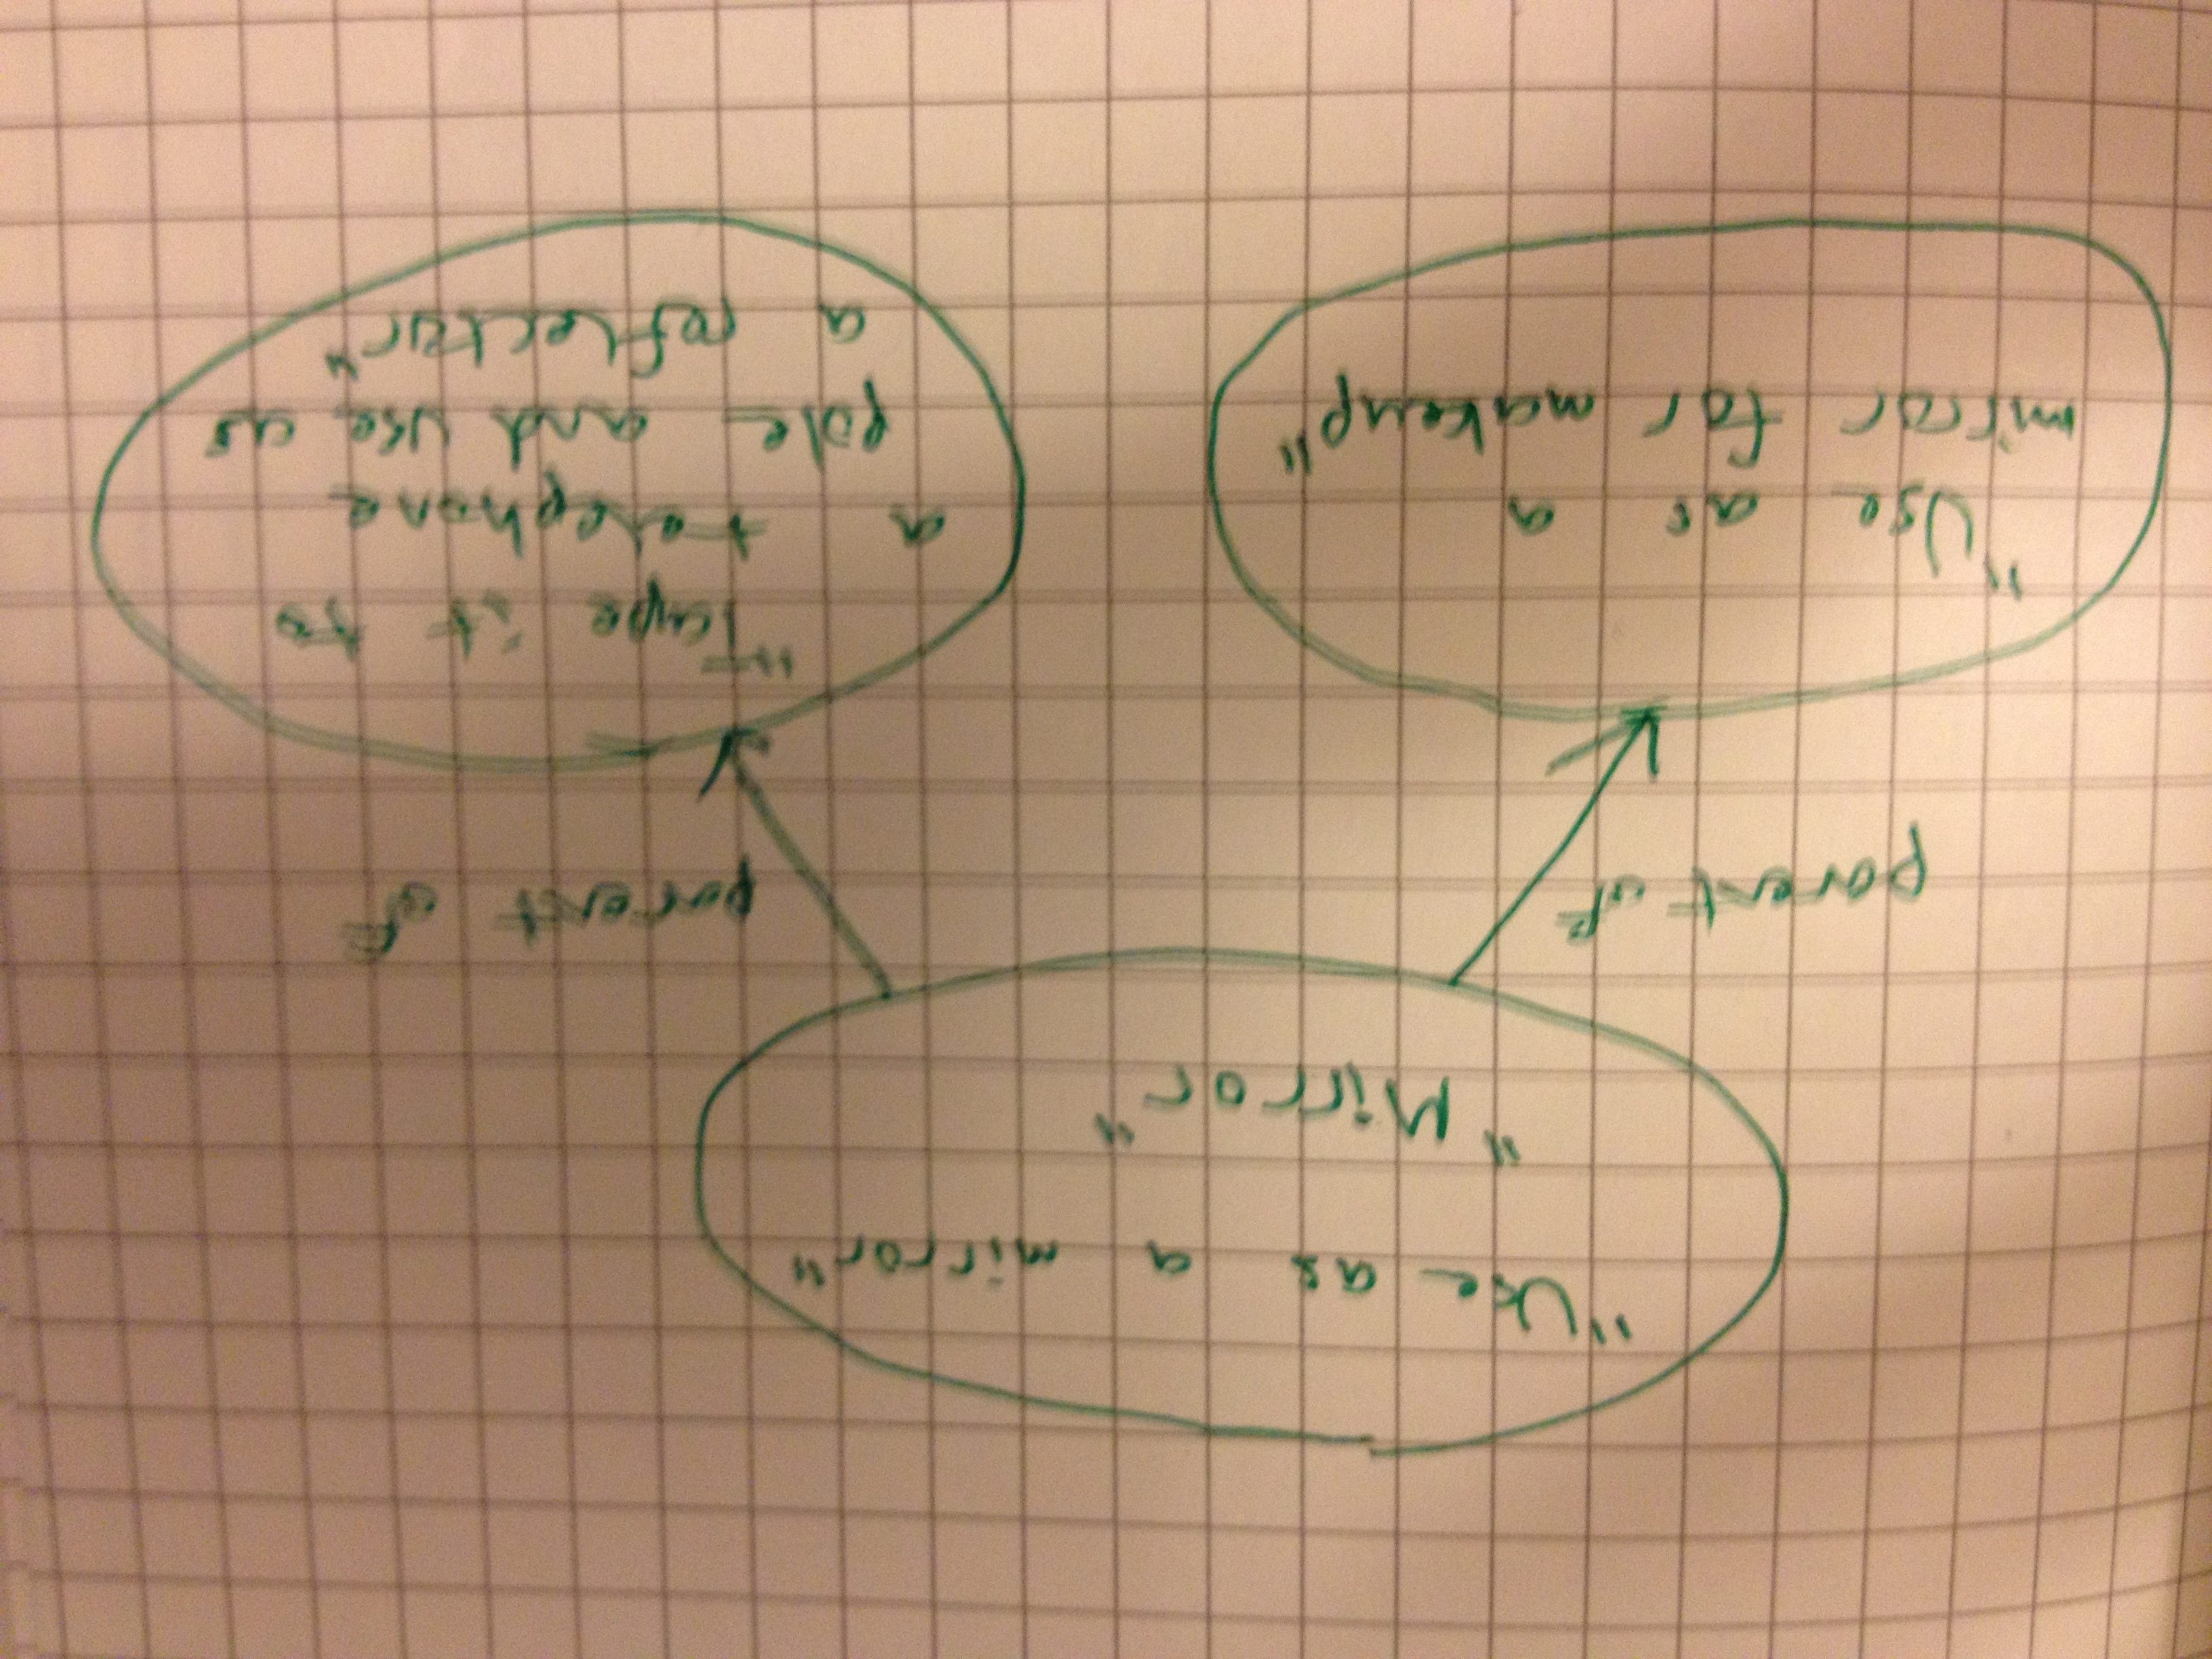
\includegraphics[width=0.9\columnwidth]{sample_category_tree}
\end{figure}

If an idea \emph{A} is a parent of idea \emph{B}, A is a generalization of B: all instances in A are are suitably general to encompass all instances in B. This difference is relative to the ideas in question.

A \emph{question forest} is simply the collection of all category trees generated in response to a particular question. Different trees in a question forest have no special relationship in meaning.

\subsection{Coding}

One researcher coded the data to produce the idea forests described above. The clustering algorithm is described in Figure FIG. Instances are added one at a time to the existing idea forest. In brief summary, the root idea that most closely matches the strategy in the instance is selected, and then that root idea and the new instance are compared in generality. This process may be repeated depending on this generality relationship, until instance is either placed in an existing idea or a new idea node is created.

The clustering algorithm relies on the human intelligence of the researcher for three key decisions:

\subsubsection{Similarity}
Two ndodes a and b have high similarity if they solve the problem in the same way, and low similarity if their solutions have no common themes. For example, in Figure FIG, "Mirror" and "Tape it to a telephone pole and use as a reflector" have high similarity, as they both solve the problem of using a broken MP3 player by using it to reflect light.

\subsubsection{Coverage}
A node a has high coverage of a node b if the problem solution in a is equal to or an abstraction of the problem solution in b. Coverage is not commutative. To return to the example, "Mirror" has high coverage of "Tape it to a telephone pole and use as a reflector", as the latter is a specific use for a mirror. On the other hand, the latter idea has low coverage of the former.

\subsubsection{Artificial Ideas}
Occasionally, two nodes have high similarity but no coverage. For example, "Use it as a mirror for makeup" and "Tape it to a telephone pole and use as a reflector" use the MP3 player in the same way, but neither is a generalization of the other. In this case, the algorithm appeals to the human coder to provide a lable for a new idea that is a generalization of both.

\begin{figure*}[h]
\begin{verbatim}
for each instance:
  idea_node = new node including instance
  current_node = root of forest
  do:
    best_match = max_similarity(idea_node, current_node.children)

    if best_match.similarity is low or current_node has no children:
      insert idea_node under current_node
      exit do
    else:
      if coverage(idea_node, best_match) == coverage(best_match, idea_node) == high:
        merge idea_node, best_match
        exit do
      else if coverage(idea_node, best_match) == coverage(best_match, idea_node) == low:
        new_parent = new artifical idea node
        insert best_match, idea_node under new_parent
        insert new_parent under current_node
        exit do
      else if coverage(idea_node, best_match) > coverage(best_match, idea_node):
        replace best_match with idea_node in tree
        current_node = idea_node
        idea_node = best_match
      else:
        current_node = best_match
\end{verbatim}
\caption{Manual clustering algorithm}
\label{fig:cluseringalg}
\end{figure*}

After completion of the coding algorithm, we were left with an idea forest as described in section SEC.


\section{Summary of Idea Forest}

The resulting forest was composed of 3007 instances, 1213 ideas, 335 category trees, and 129 non-singleton category trees. These metrics are decomposed by number condition is given in table TAB. A bird's eye view of the complete idea forest is in Figure FIG.

\begin{figure}[h!]
    \centering
    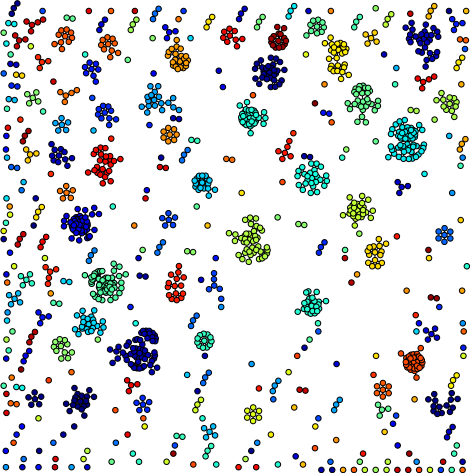
\includegraphics[width=0.9\columnwidth]{idea_forest}
    \caption{Idea Forest}
\end{figure}

\begin{table}
	\begin{tabular}[h!]{r | l l l l l l l}
	\textbf{number condition} & 5 & 10 & 20 & 50 & 75 & 100 & all \\ \hline \hline
	HITs & 57 & 47 & 23 & 10 & 10 & 10 & 146\\
	instances & 293 & 471 & 453 & 500 & 634 & 855 & 3007\\
	ideas & 171 & 249 & 278 & 341 & 443 & 177 &1212\\
	category trees & 72 & 79 & 93 & 114 & 172 & 177 &321\\
	non-singleton trees & 28 & 34 & 40 & 48 & 49 & 61 &92\\
	\end{tabular}
\end{table}

The height of category trees follows a roughly Poisson distribution, with the maximum tree height observed at 5. Summary statistics across condition are in table TAB. The third quartile drops as the number condition increases. While the upper conditions still discover categories trees with heights as great as 5, they generate many more "short" trees. This suggests that the ideas generated in the upper conditions are less common.

\begin{table}
	\begin{tabular}[h!]{r | l l l l l l l}
	\textbf{number condition} & 5 & 10 & 20 & 50 & 75 & 100 & all \\ \hline \hline
	median & 2 & 2 & 2 & 2 & 2 & 2 & 2\\
	first quartile & 2 & 2  & 1 & 1 & 1 & 1 & 1\\
	third quartile & 3 & 3 &3 &3 &2 &2 & 2\\
	\end{tabular}
	\caption{Category tree height}
\end{table}

The number of nodes and number of instances are also roughly poisson distributed (Table TAB). In keeping with the findings for height, trees found in the upper number conditions are smaller than trees found in the lower conditions. The precipitous drop in median tree size suggests that in the largest condition, participants are finding rare ideas with only a few variants and less than 14 instances.

\begin{table}
\begin{tabular}[h!]{r | l l l l l l l}
	\textbf{number condition} & 5 & 10 & 20 & 50 & 75 & 100 & all \\ \hline \hline
	number of nodes& \\ \hline
    median &5&5&4&3&2&2&2 \\
	first quartile &2&2&1&1&1&1&1 \\
	third quartile &17&17&14&10&5&5&5 \\
	number of instances& \\ \hline
	median &14&14&12&10&4&4&4 \\
    first quartile &4&4&4&2&1&1&1 \\
	third quartile &47&45&30&23&13&13&13 \\
	\end{tabular}
	\caption{Number of ideas and instances in trees}
\end{table}

To better understand what this distribution of tree sizes means...




% Stupid citation so latex will stop complaining
\cite{yu_internet-scale_2013}

% Balancing columns in a ref list is a bit of a pain because you
% either use a hack like flushend or balance, or manually insert
% a column break.  http://www.tex.ac.uk/cgi-bin/texfaq2html?label=balance
% multicols doesn't work because we're already in two-column mode,
% and flushend isn't awesome, so I choose balance.  See this
% for more info: http://cs.brown.edu/system/software/latex/doc/balance.pdf
%
% Note that in a perfect world balance wants to be in the first
% column of the last page.
%
% If balance doesn't work for you, you can remove that and
% hard-code a column break into the bbl file right before you
% submit:
%
% http://stackoverflow.com/questions/2149854/how-to-manually-equalize-columns-
% in-an-ieee-paper-if-using-bibtex
%
% Or, just remove \balance and give up on balancing the last page.
%
\balance

\bibliographystyle{acm-sigchi}
\bibliography{paper}
\end{document}
